\documentclass[presentation,english,usenames,dvipsnames]{beamer}
\usepackage[utf8]{inputenc}
\usepackage{babel}
\usepackage{graphicx}
\usepackage{longtable}
\usepackage{float}
\usepackage{wrapfig}
\usepackage{soul}
\usepackage{textcomp}
\usepackage{marvosym}
\usepackage{wasysym}
\usepackage{latexsym}
\usepackage{amssymb}
\usepackage{hyperref}
\tolerance=1000
\usepackage{listings}
\usepackage[iso]{isodate}
\usepackage[font=scriptsize, skip=0pt]{caption}
\usepackage[font=scriptsize, skip=0pt]{subcaption}
\usepackage{pgfplots, pgfplotstable}
\pgfplotsset{compat=1.14}
\usepackage{tikz}
\usetikzlibrary{fit, shapes}
\pgfdeclarelayer{background}
\pgfsetlayers{background,main}

\title[Peer-to-Peer Incentives]{Incentivizing Peers to Contribute in a
Low-Latency Name-Lookup Service}
\author{Marc Lehmann}
\subtitle{Final Master Talk}
\date{\today}


\usetheme{Comsys}
% Adjust the title font size, because my title spans 3 lines otherwise.
\setbeamerfont{title}{size*={16}{26.4},series=\bfseries}

\begin{document}

\setbeamertemplate{footline}[empty]
\begin{frame}
  \titlepage
\end{frame}

\setbeamertemplate{footline}[comsys]

\begin{frame}{Motivation}
  \begin{itemize}
    \item Name-mapping service important to facilitate communication
    \begin{itemize}
      \item names to IPs (DNS)
      \item people to devices (instant messaging)
    \end{itemize}
    \item Think of a peer-to-peer chat system

    \pause

    \item Privacy concerns in centralized systems
    \begin{itemize}
      \item Server gets a lot of information about whom a user communicates with
      \item Can build user profiles
      \item Can become target for others who want to build profiles
    \end{itemize}
    \item Spread requests to many different nodes in a DHT
    \item Requires lots of nodes
  \end{itemize}

  \pause

  \begin{block}{}
    Users need to participate themselves, everyone stores a few records
  \end{block}
\end{frame}

\begin{frame}{Encouraging peers to contribute}
  \begin{itemize}
    \item Assume peers are selfish, don't want to invest resources
    \item Only leverage: users want good service
    \item Give bad peers bad service (delayed responses)

    \pause

    \item Track how good peers are via a reputation system (points)
    \item Existing solutions to track reputation insufficient
    \begin{itemize}
      \item Assume a central authority {\color{gray}\tiny[Gupta et al.]}
      \item Aren't Scalable {\color{gray}\tiny[Zhou et al.]}
      \item Or propose using another DHT {\color{gray}\tiny[Feldman et al.]},
            introducing additional latency
    \end{itemize}

    \pause

  \end{itemize}
  \begin{block}{}
    Create small, overlapping subsets of peers (query groups), broadcast
    reputation updates in those
  \end{block}
\end{frame}

\begin{frame}{Query Groups}
  \begin{minipage}{0.5\textwidth}
    \begin{itemize}
      \item Using Chord to illustrate
      \item Need to be able to reach peers in finger table
      \item Need to share a query group with each of these peers
      \item (Not necessarily the same for all)
    \end{itemize}
  \end{minipage}% This comment is necessary to remove any space between the minipages
  \begin{minipage}{0.5\textwidth}
    \begin{figure}
      \centering
      \begin{tikzpicture}
        \begin{scope}[every node/.style={
          circle,
          fill=black,
          inner sep=0pt,
          minimum size=5pt
          }]
          \node[minimum size=8pt] (A) at (90:2) {};
          \node[red] (B) at (30:2) {};
          \node[blue] (C) at (330:2) {};
          \node[violet] (D) at (270:2) {};
          \node[OliveGreen] (E) at (210:2) {};
          \node (F) at (150:2) {};
        \end{scope}

        \draw (B) -- (C)[draw=none] node[midway, sloped] {\ldots};
        \draw (C) -- (D)[draw=none] node[midway, sloped] {\ldots};
        \draw (D) -- (E)[draw=none] node[midway, sloped] {\ldots};
        \draw (E) -- (F)[draw=none] node[midway, sloped] {\ldots};
        \draw (F) -- (A)[draw=none] node[midway, sloped] {\ldots};

        \draw[->] (A) -- (B);
        \draw[->] (A) -- (C);
        \draw[->] (A) -- (D);
        \draw[->] (A) -- (E);

        \begin{pgfonlayer}{background}
          \begin{scope}[every node/.style={
            ellipse,
            draw=black,
            thick,
            inner sep=0pt,
            inner xsep=0pt,
            inner ysep=0pt,
            opacity=0.5
          }]
            \invisible{
              \node[fit=(A)(B), fill=red!30, rotate=-30] {};
            }
            \invisible{
              \node[fit=(A)(C)(D), fill=violet!30, rotate=18, xshift=-15pt] {};
            }
            \invisible{
              \node[fit=(A)(E), fill=OliveGreen!30, rotate=-30,
                    inner xsep=-15pt] {};
            }
          \end{scope}
        \end{pgfonlayer}
      \end{tikzpicture}
    \end{figure}
  \end{minipage}
\end{frame}

\begin{frame}{Query Groups}
  \begin{minipage}{0.5\textwidth}
    \begin{itemize}
      \item \visible<1->{Join query group with red peer}
      \item \visible<2->{Join query group with blue peer}
      \item \visible<2->{Purple peer is also in that group}
      \item \visible<3->{Join query group with green peer}
    \end{itemize}
  \end{minipage}% This comment is necessary to remove any space between the minipages
  \begin{minipage}{0.5\textwidth}
    \begin{figure}
      \centering
      \begin{tikzpicture}
        \begin{scope}[every node/.style={
          circle,
          fill=black,
          inner sep=0pt,
          minimum size=5pt
          }]
          \node[minimum size=8pt] (A) at (90:2) {};
          \node[red] (B) at (30:2) {};
          \node[blue] (C) at (330:2) {};
          \node[violet] (D) at (270:2) {};
          \node[OliveGreen] (E) at (210:2) {};
          \node (F) at (150:2) {};
        \end{scope}

        \draw (B) -- (C)[draw=none] node[midway, sloped] {\ldots};
        \draw (C) -- (D)[draw=none] node[midway, sloped] {\ldots};
        \draw (D) -- (E)[draw=none] node[midway, sloped] {\ldots};
        \draw (E) -- (F)[draw=none] node[midway, sloped] {\ldots};
        \draw (F) -- (A)[draw=none] node[midway, sloped] {\ldots};

        \draw[->] (A) -- (B);
        \draw[->] (A) -- (C);
        \draw[->] (A) -- (D);
        \draw[->] (A) -- (E);

        \begin{pgfonlayer}{background}
          \begin{scope}[every node/.style={
            ellipse,
            draw=black,
            thick,
            inner sep=0pt,
            inner xsep=0pt,
            inner ysep=0pt,
            opacity=0.5
          }]
            \visible<1->{
              \node[fit=(A)(B), fill=red!30, rotate=-30] {};
            }
            \visible<2->{
              \node[fit=(A)(C)(D), fill=violet!30, rotate=18, xshift=-15pt] {};
            }
            \visible<3->{
              \node[fit=(A)(E), fill=OliveGreen!30, rotate=-30,
                    inner xsep=-15pt] {};
            }
          \end{scope}
        \end{pgfonlayer}
      \end{tikzpicture}
    \end{figure}
  \end{minipage}
\end{frame}

\begin{frame}{Query Groups}
  \begin{minipage}{0.5\textwidth}
    \begin{itemize}
      \item Query groups also contain other peers
      \item They are the peers we forward queries to
      \item Everybody knows everybody's reputation
    \end{itemize}
  \end{minipage}% This comment is necessary to remove any space between the minipages
  \begin{minipage}{0.5\textwidth}
    \begin{figure}
      \centering
      \begin{tikzpicture}
        \begin{scope}[every node/.style={
          circle,
          fill=black,
          inner sep=0pt,
          minimum size=5pt
          }]
          \node[minimum size=8pt] (A) at (90:2) {};
          \invisible{\node[red] (B) at (30:2) {};}
          \node[blue] (C) at (330:2) {};
          \node[violet] (D) at (270:2) {};
          \invisible{\node[OliveGreen] (E) at (210:2) {};}
          \invisible{\node (F) at (150:2) {};}
        \end{scope}
        \begin{scope}[every node/.style={
          circle,
          draw=black,
          inner sep=0pt,
          minimum size=5pt
          }]
          \node (G) at (90:1) {};
          \node (H) at (180:0.5) {};
          \node (I) at (135:1.2) {};
          \node (J) at (280:1.3) {};
          \node (K) at (0:1) {};
          \node (L) at (330:1) {};
        \end{scope}

        \draw (A) -- (C)[draw=gray, opacity=0.8];
        \draw (A) -- (D)[draw=gray, opacity=0.8];
        \draw (A) -- (G)[draw=gray, opacity=0.8];
        \draw (A) -- (H)[draw=gray, opacity=0.8];
        \draw (A) -- (I)[draw=gray, opacity=0.8];
        \draw (A) -- (J)[draw=gray, opacity=0.8];
        \draw (A) -- (K)[draw=gray, opacity=0.8];
        \draw (A) -- (L)[draw=gray, opacity=0.8];
        \draw (C) -- (D)[draw=gray, opacity=0.8];
        \draw (C) -- (G)[draw=gray, opacity=0.8];
        \draw (C) -- (H)[draw=gray, opacity=0.8];
        \draw (C) -- (I)[draw=gray, opacity=0.8];
        \draw (C) -- (J)[draw=gray, opacity=0.8];
        \draw (C) -- (K)[draw=gray, opacity=0.8];
        \draw (C) -- (L)[draw=gray, opacity=0.8];
        \draw (D) -- (G)[draw=gray, opacity=0.8];
        \draw (D) -- (H)[draw=gray, opacity=0.8];
        \draw (D) -- (I)[draw=gray, opacity=0.8];
        \draw (D) -- (J)[draw=gray, opacity=0.8];
        \draw (D) -- (K)[draw=gray, opacity=0.8];
        \draw (D) -- (L)[draw=gray, opacity=0.8];
        \draw (G) -- (H)[draw=gray, opacity=0.8];
        \draw (G) -- (I)[draw=gray, opacity=0.8];
        \draw (G) -- (J)[draw=gray, opacity=0.8];
        \draw (G) -- (K)[draw=gray, opacity=0.8];
        \draw (G) -- (L)[draw=gray, opacity=0.8];
        \draw (H) -- (I)[draw=gray, opacity=0.8];
        \draw (H) -- (J)[draw=gray, opacity=0.8];
        \draw (H) -- (K)[draw=gray, opacity=0.8];
        \draw (H) -- (L)[draw=gray, opacity=0.8];
        \draw (I) -- (J)[draw=gray, opacity=0.8];
        \draw (I) -- (K)[draw=gray, opacity=0.8];
        \draw (I) -- (L)[draw=gray, opacity=0.8];
        \draw (J) -- (K)[draw=gray, opacity=0.8];
        \draw (J) -- (L)[draw=gray, opacity=0.8];
        \draw (K) -- (L)[draw=gray, opacity=0.8];

        \invisible{\draw (B) -- (C)[draw=none] node[midway, sloped] {\ldots};}
        \invisible{\draw (C) -- (D)[draw=none] node[midway, sloped] {\ldots};}
        \invisible{\draw (D) -- (E)[draw=none] node[midway, sloped] {\ldots};}
        \invisible{\draw (E) -- (F)[draw=none] node[midway, sloped] {\ldots};}
        \invisible{\draw (F) -- (A)[draw=none] node[midway, sloped] {\ldots};}

        \invisible{\draw[->] (A) -- (B);}
        \invisible{\draw[->] (A) -- (C);}
        \invisible{\draw[->] (A) -- (D);}
        \invisible{\draw[->] (A) -- (E);}

        \begin{pgfonlayer}{background}
          \begin{scope}[every node/.style={
            ellipse,
            draw=black,
            thick,
            inner sep=0pt,
            inner xsep=0pt,
            inner ysep=0pt,
            opacity=0.5
          }]
            \invisible{
              \node[fit=(A)(B), fill=red!30, rotate=-30] {};
            }
            \node[fit=(A)(C)(D), fill=violet!30, rotate=18, xshift=-15pt] {};
            \invisible{
              \node[fit=(A)(E), fill=OliveGreen!30, rotate=-30,
                    inner xsep=-15pt] {};
            }
          \end{scope}
        \end{pgfonlayer}
      \end{tikzpicture}
    \end{figure}
  \end{minipage}
\end{frame}

\begin{frame}{Reputation}
  \begin{itemize}
    \item If reputation is low, responses deliberately delayed
    \begin{itemize}
      \item Above a \emph{penalty threshold}, no delays
      \item Below, delay proportional to distance to the threshold
      \begin{itemize}
        \item 10 reputation $\rightarrow$ no delay
        \item 9 reputation $\rightarrow$ 1s delay
        \item 7.5 reputation $\rightarrow$ 2.5s delay
      \end{itemize}
    \end{itemize}

    \pause

    \item Earn reputation for responding to queries (+1)
    \item Lose reputation for not responding (in time) (-2)

    \pause

    \item Peers want fast responses to their queries
    \begin{itemize}
      \item Incentive to respond in time
    \end{itemize}
  \end{itemize}
\end{frame}

\begin{frame}{Main problems}
  \begin{itemize}
    \item Reputation availability
    \begin{itemize}
      \item Good peers need the ability to gain enough reputation
    \end{itemize}
    \item Complaint system
    \begin{itemize}
      \item Disagreements between peers where there is no proof
      \item Must not be able to exploit the system by lying
    \end{itemize}
    \item Query group management
    \begin{itemize}
      \item Creating, joining, leaving
      \item Can everyone find the groups he needs?
    \end{itemize}
  \end{itemize}

  \pause

  \begin{block}{}
    Investigated reputation availability
  \end{block}
\end{frame}

\begin{frame}{Simulation}
  \begin{itemize}
    \item Discrete event simulation in SimPy
    \item Simplified implementation of the system

    \pause

    \item Peers are lazy, but want delay-free responses
    \begin{itemize}
      \item Do their best to cooperate until \emph{saturation reputation} (14)
      \item Penalty threshold plus buffer, tolerate unintentional misbehavior

      \pause

      \item Once they reach it, ignore the next query so they're below it again
      \item Timeout at sender, retry another peer if possible
    \end{itemize}

    \pause

    \item Requests generated externally, one per second per peer
  \end{itemize}
\end{frame}

\begin{frame}{Peer selection}
  \begin{itemize}
    \item Access record in the DHT $\rightarrow$ need to send query to query
    peer
    \item Choice of recipient has an impact on reputation distribution

    \pause

    \item First rule: select the query peer closest to the target
    \begin{itemize}
      \item Distance metric peer $\rightarrow$ key
    \end{itemize}
  \end{itemize}

    \pause

  \begin{block}{}
    If multiple, no tie breaker
  \end{block}
\end{frame}

\begin{frame}{Peer selection: closest, no tie breaker}
  \begin{figure}
    \centering
    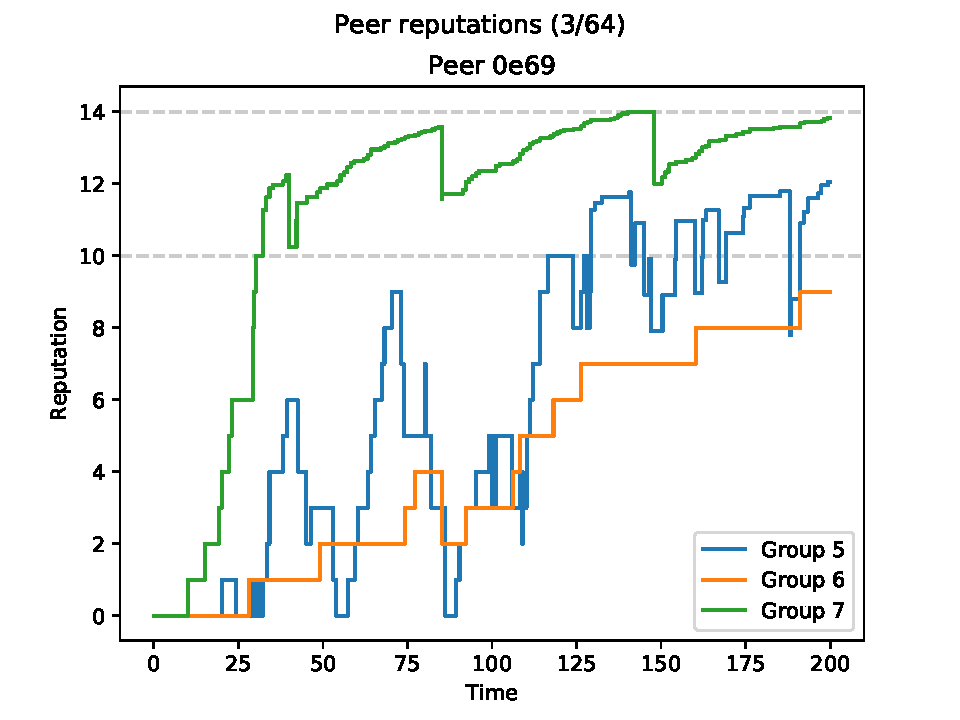
\includegraphics[width=0.5\textwidth]{figures/selection_overlap_peer_reps_3_of_64}%
    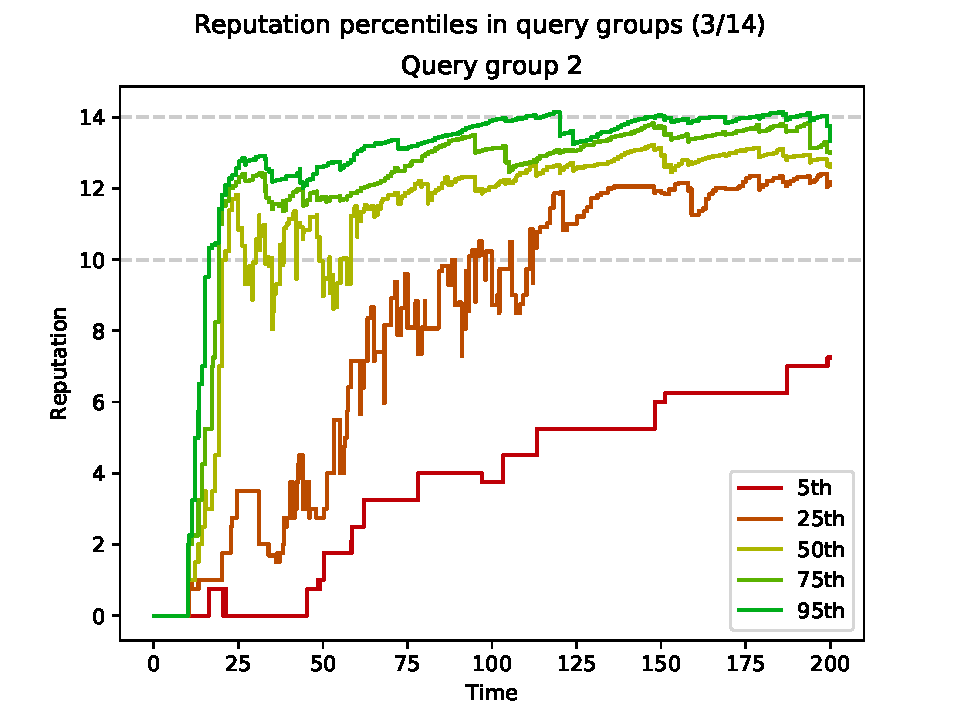
\includegraphics[width=0.5\textwidth]{figures/selection_overlap_rep_percs_3_of_14}
  \end{figure}
\end{frame}

\begin{frame}{Peer selection: closest, no tie breaker}
  \begin{itemize}
    \item Peers selected in same order
    \item Unlucky peers are second choice, only selected when first choice peer
          doesn't respond
    \item Difficult for them to gain reputation
    \item Same iteration order, copied from peer to peer
    \item Could also happen in a real system
  \end{itemize}

  \pause

  \begin{block}{}
    Modification: if multiple viable peers, use the one with lowest reputation
  \end{block}
\end{frame}

\begin{frame}{Peer selection: closest $\rightarrow$ lowest reputation}
  \begin{minipage}{0.5\textwidth}
    \begin{figure}
      \centering
      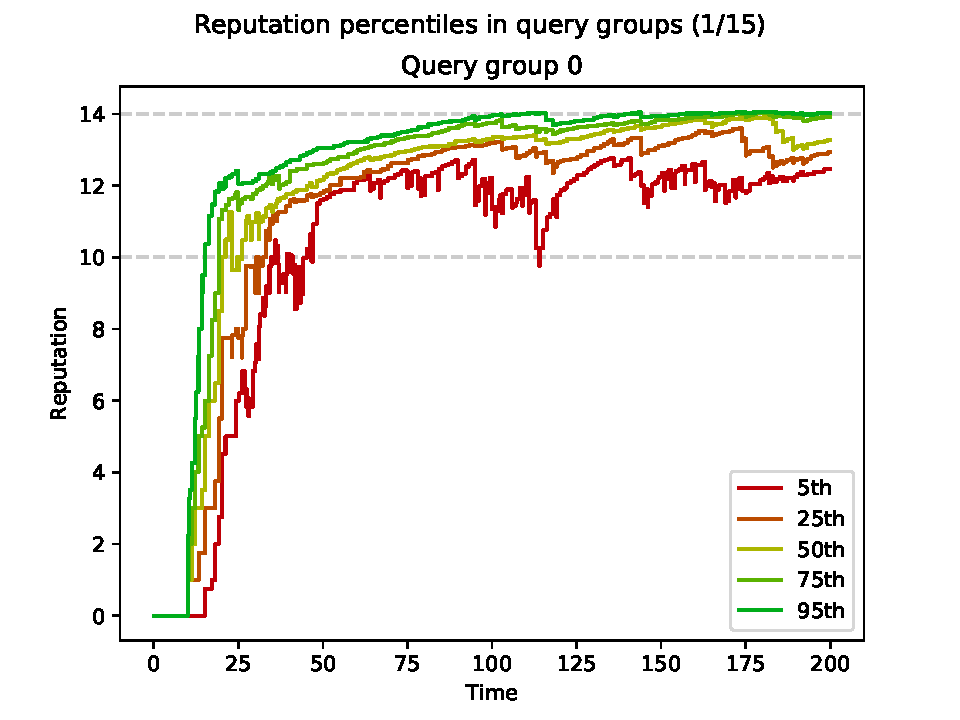
\includegraphics[width=1\textwidth]{figures/selection_overlap_rep_sorted_rep_percs_1_of_15}
    \end{figure}
  \end{minipage}%
  \begin{minipage}{0.5\textwidth}
    \begin{itemize}
      \item Better distribution of reputation
      \item But no incentive, must be enforced with threat of penalty
      \item Not so simple, need to detect it
    \end{itemize}
  \end{minipage}
\end{frame}

\begin{frame}{Reputation attenuation}
  \begin{itemize}
    \item Reputation attenuation also very important
    \item Was turned on, without it peer reps look like this
  \end{itemize}

  \pause

  \begin{minipage}{0.5\textwidth}
    \begin{figure}
      \centering
      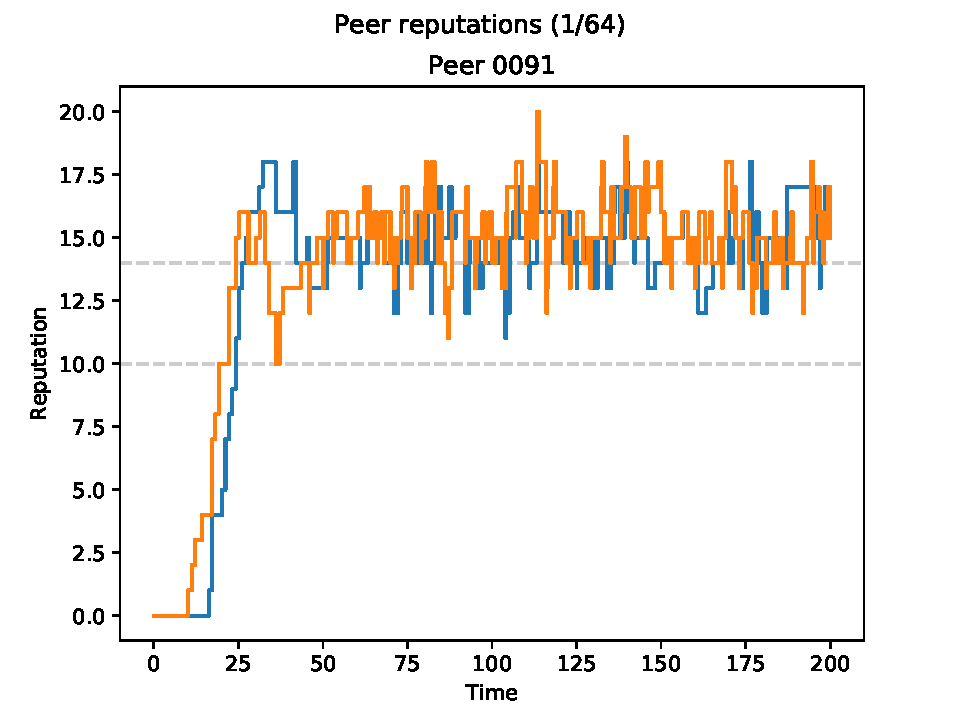
\includegraphics[width=1\textwidth]{figures/attenuation_no_attenuation_peer_reps_1_of_64}
    \end{figure}
  \end{minipage}%
  \begin{minipage}{0.5\textwidth}
    \begin{itemize}
      \item Reputation for response: +1
      \item Reputation for timeout: -2
      \item Respond twice, timeout once
    \end{itemize}
  \end{minipage}
\end{frame}

\begin{frame}{Reputation attenuation}
  \begin{itemize}
    \item Reward and penalty determine number of timeouts
    \item Want peers to respond more often
    \item Smaller reward or bigger penalty

    \pause

    \begin{itemize}
      \item Difficult to gain reputation for newcomers, long time with bad
            service
    \end{itemize}

    \pause

    \item Give peers reputation to begin with

    \pause

    \begin{itemize}
      \item Enables whitewashing: make new ID, rejoin
    \end{itemize}

    \pause

  \end{itemize}
  \begin{block}{}
    Make it harder to gain reputation above the penalty threshold
  \end{block}
\end{frame}

\begin{frame}{Reputation attenuation}
  \begin{itemize}
    \item Two kinds of reputation
    \begin{itemize}
      \item Raw reputation $r_r$
      \item Effective reputation, generated from raw reputation by attenuating
    \end{itemize}

    \pause

    \item Linear until the penalty threshold, root-ish after
    \item Only increases attenuated
  \end{itemize}
  \begin{minipage}{0.5\textwidth}
    \vspace{6.2mm}
    \begin{figure}
      \begin{tikzpicture}
        \begin{axis}[
          xlabel=$r_r$,
          ylabel={$att(r_r)$},
          xmin=0,
          xmax=75,
          ymin=0,
          ymax=20,
          width=0.9\columnwidth
        ]
          \addplot[domain=0:75, samples=751]{min(min(x, 10) + max(x - 10, 0) ^
          0.35, 15)}; \end{axis}
      \end{tikzpicture}
    \end{figure}

    \pause

  \end{minipage}%
    \begin{minipage}{0.5\textwidth}
    \begin{figure}
      \centering
      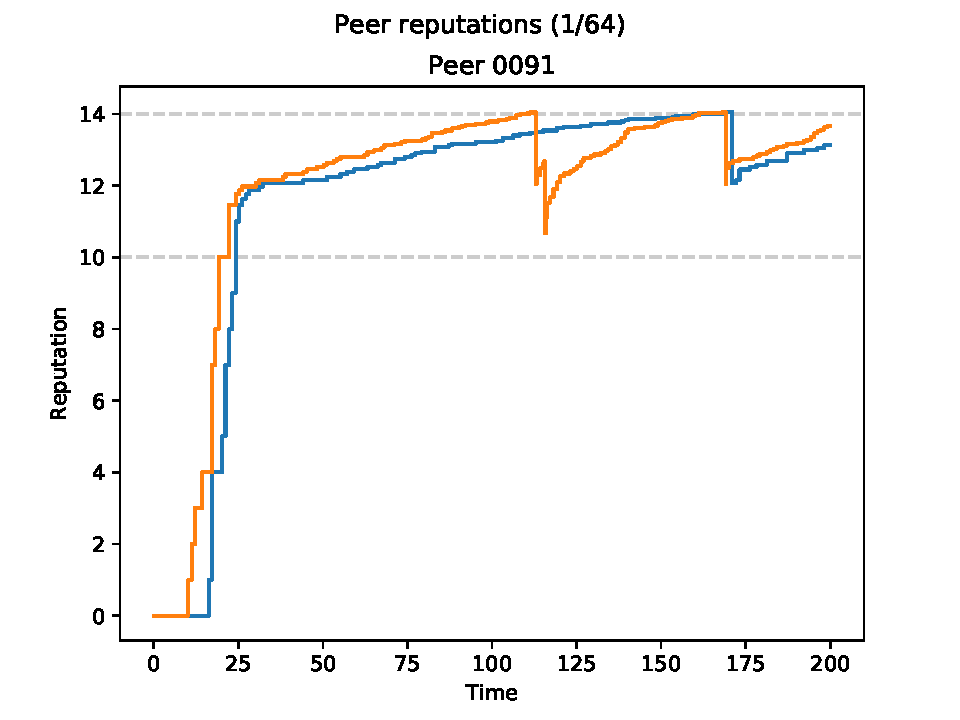
\includegraphics[width=1\textwidth]{{{figures/attenuation_0.35_1_exponential_peer_reps_1_of_64}}}
    \end{figure}
  \end{minipage}
\end{frame}

\begin{frame}{Reputation attenuation}
  \begin{itemize}
    \item Doesn't hinder newcomers
    \item Can control how often peers ignore queries

    \pause

    \item Also ensures continuous cooperation
    \item Can't earn lots of reputation, then leech

    \pause

    \item But makes it more difficult the more reputation you have
    \begin{itemize}
      \item Disadvantage for peers with higher saturation
    \end{itemize}
  \end{itemize}
\end{frame}

\begin{frame}{Recursive query problem}
  \begin{figure}
    \centering
    \begin{tikzpicture}
      \begin{scope}[every node/.style={
        rectangle,
        draw,
        font=\scriptsize
      }]
        \node (A) at (-2.5, 0) {red: 10};
        \node (B)[align=left] at (0, 0) {red: 10\\purple: 6};
        \node (C) at (2.5, 0) {purple: 10};
      \end{scope}

      \begin{scope}[every node/.style={
        font=\scriptsize,
        midway
      }]
        \path (A) edge[->, above, bend left=30] node
            {\textbf{1:} query at 0} (B);
        \visible<2->{
          \path (B) edge[->, above, bend left=30] node
            {\textbf{2:} query at 0.1} (C);
        }
        \visible<3->{
          \path (C) edge[->, below, bend left=30] node
            {\textbf{3:} response at 4.1} (B);
        }
        \visible<4->{
          \path (B) edge[->, below, bend left=30] node[align=left]
            {\textbf{4:} response at 4.2,\\too late} (A);
        }
      \end{scope}

      \begin{pgfonlayer}{background}
        \begin{scope}[every node/.style={
          circle,
          inner sep=0,
          inner xsep=0.3cm,
          inner ysep=0pt,
          opacity=0.5
        }]
          \node[fit=(A)(B), fill=red!30, rotate=0,
                label={[label distance=-1cm]90:\scriptsize query group 1}] {};
          \node[fit=(B)(C), fill=violet!30, rotate=0,
                label={[label distance=-1cm]90:\scriptsize query group 2}] {};
        \end{scope}
      \end{pgfonlayer}
    \end{tikzpicture}
  \end{figure}
  \visible<5->{
    \begin{itemize}
      \item Penalty threshold: 10
      \item Middle peer: low reputation, can't respond in time
    \end{itemize}
  }
\end{frame}

\begin{frame}{Recursive query problem}
  \begin{figure}
    \centering
    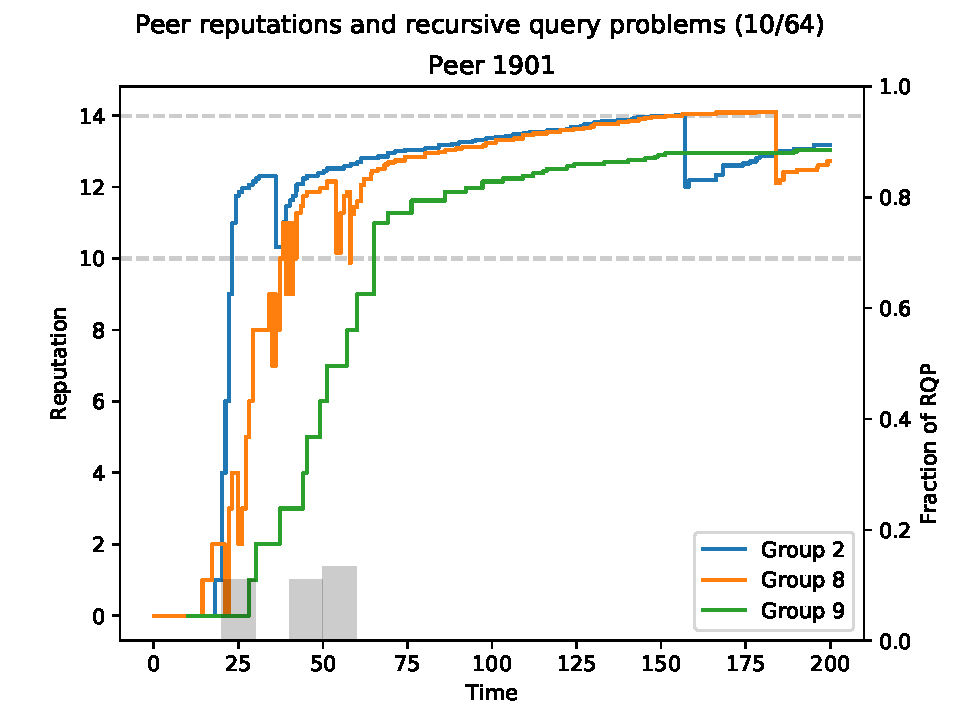
\includegraphics[width=0.5\textwidth]{figures/selection_overlap_rep_sorted_peer_reps_with_rqp_10_of_64}
  \end{figure}
  \begin{itemize}
    \item Orange group struggles while green group causes delays
    \item Once all are above the threshold, no problem anymore
    \item Inherent to the system
  \end{itemize}
\end{frame}

\begin{frame}
- performance? need to explain routing in detail
  \begin{itemize}
    \item
  \end{itemize}
\end{frame}

\begin{frame}{Conclusion}
  \begin{itemize}
    \item Want to get users to participate in a DHT
    \item Reputation system, need to respond to get fast responses
    \item Small query groups to spread reputation updates
    \item Reputation availability: $\checkmark$
    \begin{itemize}
      \item Need to enforce choosing lowest-reputation of viable peers
      \item Reputation must be attenuated above the penalty threshold
    \end{itemize}
    \item Other problems need to be investigated
    \begin{itemize}
      \item Complaint system
      \item Query group management
    \end{itemize}
  \end{itemize}
\end{frame}

\begin{frame}
\end{frame}

\begin{frame}{Reputation Updates}
  \begin{itemize}
    \item Timeout or late/early response
    \begin{itemize}
      \item Sender broadcasts a reputation decrease
      \item Gets a little reputation for doing so
    \end{itemize}
    \item Successful query
    \begin{itemize}
      \item Sender gives the responder a \emph{cooperation confirmation}
      \item Responder broadcasts it, increasing his own reputation
      \item No cooperation confirmation $\rightarrow$ complaint system
    \end{itemize}
  \end{itemize}
\end{frame}

\begin{frame}{Query Groups (Kademlia/P-Grid)}
  \begin{itemize}
    \item View keys as bit string
    \item Peers have a routing prefix (bit string): store keys that start with
          that prefix
    \item Peers are in contact with others with the same routing prefix
          (replication)
    \item Other routing prefixes: know other peers closer to them
  \end{itemize}
  \begin{figure}
    \centering
    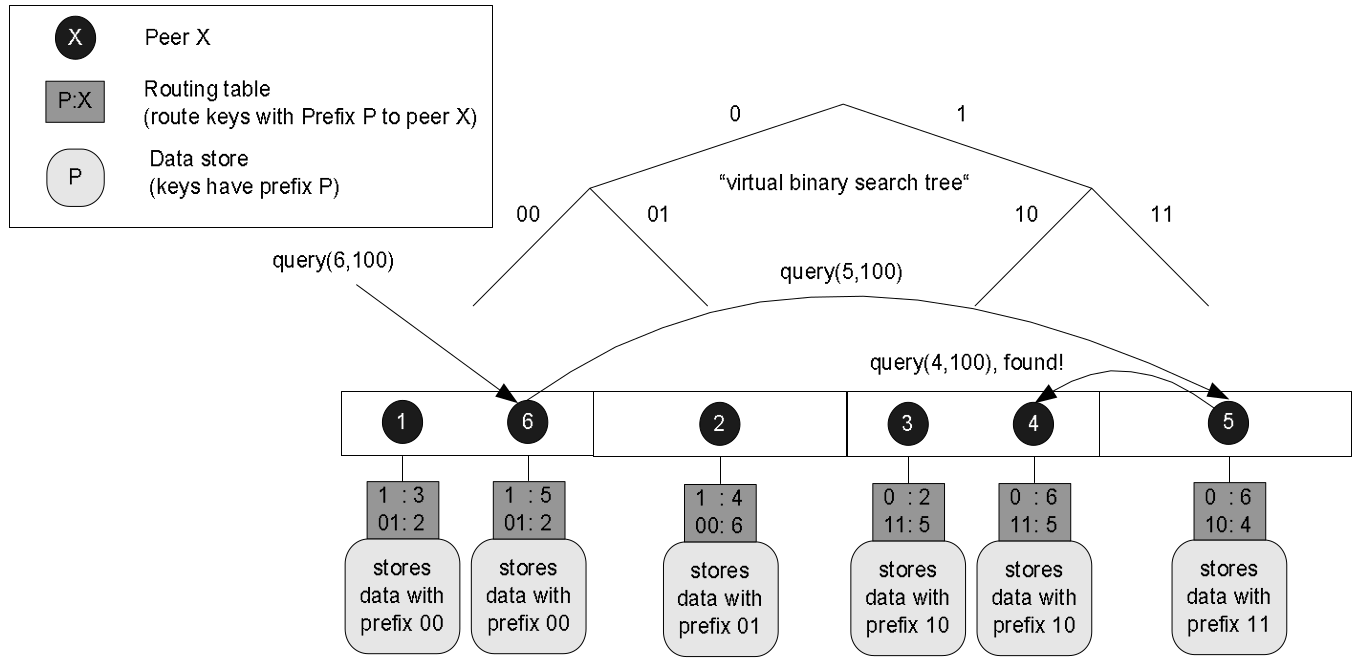
\includegraphics[width=0.5\textwidth]{figures/p-grid}
    \caption*{\tiny From \emph{P-Grid: A Self-organizing Structured P2P System}}
  \end{figure}
\end{frame}

\begin{frame}{Query Groups (Kademlia/P-Grid)}
  \begin{itemize}
    \item Dashed: Same routing prefix, replication (sync groups)
    \item Solid: Query groups
  \end{itemize}
  \begin{figure}
    \centering
    \begin{tikzpicture}
      \begin{scope}[every node/.style={draw}]
        \node[color=red] (A) at (0:2) {P: 001};
        \node[color=blue] (B) at (45:2) {P: 001};
        \node[color=red] (C) at (90:2) {P: 001};
        \node[color=blue] (D) at (135:2) {P: 010};
        \node[color=OliveGreen] (E) at (180:2) {P: 010};
        \node[color=blue] (F) at (225:2) {P: 101};
        \node[color=red] (G) at (270:2) {P: 101};
        \node[color=OliveGreen] (H) at (315:2) {P: 101};
      \end{scope}

      \path (A) edge[thick,dashed,bend right=15] (B);
      \path (B) edge[thick,dashed,bend right=15] (C);
      \path (A) edge[thick,dashed,bend left=15] (C);
      \path (D) edge[thick,dashed,bend right=15] (E);
      \path (F) edge[thick,dashed,bend right=15] (G);
      \path (G) edge[thick,dashed,bend right=15] (H);
      \path (F) edge[thick,dashed,bend left=15] (H);
      \path (A) edge[thick,color=red,bend left=20] (C);
      \path (C) edge[thick,color=red] (G);
      \path (A) edge[thick,color=red,bend right=15] (G);
      \path (B) edge[thick,color=blue] (D);
      \path (D) edge[thick,color=blue,bend left=15] (F);
      \path (B) edge[thick,color=blue] (F);
      \path (E) edge[thick,color=OliveGreen] (H);
    \end{tikzpicture}
  \end{figure}
\end{frame}

\begin{frame}{Why do we need incentives?}
  \begin{itemize}
    \item Maybe we don't
    \item "Just distribute software that contributes to the DHT, people will be
          too lazy to change it for a small benefit"
          \begin{itemize}
            \item Some alternative implementation may opt to leave it out
            \item Maybe for performance, maybe for security
          \end{itemize}
    \item Assume the worst case, be ready for reality
    \item Just nice to know if it would work
  \end{itemize}
\end{frame}

\end{document}
